\block{Motivation}{
          \begin{tikzfigure}[]
    
            \begin{minipage}{.32\linewidth}
              \centering
              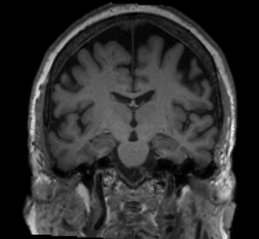
\includegraphics[height=9cm]{Figures/Brain__1.CN.png}
              \caption{\textcolor{col_CN}{CN}}
            \end{minipage}%
            \begin{minipage}{.32\linewidth}
              \centering
              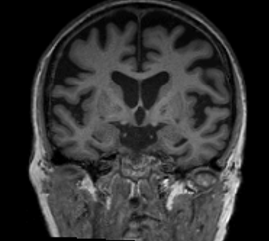
\includegraphics[height=9cm]{Figures/Brain__2.MCI.png}
              \caption{\textcolor{col_MCI}{MCI}}
            \end{minipage}
            \begin{minipage}{.32\linewidth}
              \centering
              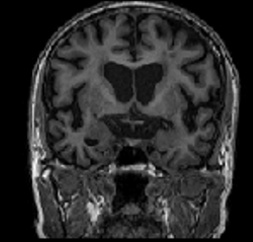
\includegraphics[height=9cm]{Figures/Brain__3.AD.png}
              \caption{\textcolor{col_AD}{Dementia}}
            \end{minipage}
            \end{tikzfigure}

        
        \begin{itemize}
            \item Dementia shows 3 progressive stages.

            \begin{itemize}
             \item \textcolor{col_CN}{CN} : Cognitively Normal

             \item \textcolor{col_MCI}{MCI} : Mild Cognitive Impairment

            \item \textcolor{col_AD}{Dementia} : Most of them were Alzheimer's Disease
             
            \end{itemize}
            
            \item Each stage shows different \textbf{brain atrophy}.

            \item Hence, their \textbf{functional activity} from resting-state fMRI (RS-fMRI) should be different.

            
                      
          \end{itemize}
        
        
}